\documentclass{article}
\usepackage{tikz}
\usetikzlibrary{arrows}

\begin{document}

\begin{figure}
\begin{center}
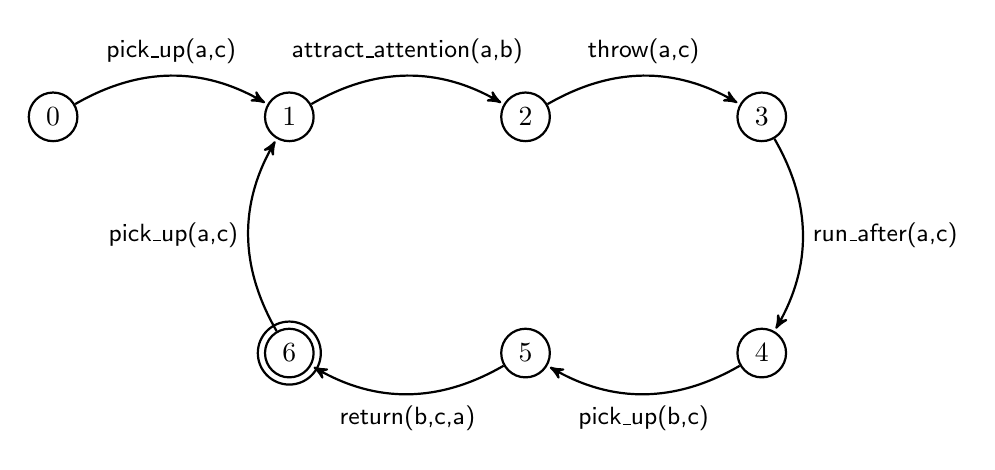
\begin{tikzpicture}[->,>=stealth',shorten >=1pt,auto,node distance=3cm,minimum size=.6cm,
  thick,main node/.style={circle,draw}]

  \node[main node] (0) {0};
  \node[main node] (1) [right of=0] {1};
  \node[main node] (2) [right of=1] {2};
  \node[main node] (3) [right of=2] {3};
  \node[main node] (4) [below of=3] {4};
  \node[main node] (5) [below of=2] {5};
\draw[thick,fill=white] (3,-3) circle (.4cm); 
  \node[main node] (6) [below of=1] {6};


  \path[every node/.style={font=\sffamily\small}]
    (0) edge [bend left] node {pick\_up(a,c)} (1)
    (1) edge [bend left] node {attract\_attention(a,b)} (2)
    (2) edge [bend left] node {throw(a,c)} (3)
    (3) edge [bend left] node {run\_after(a,c)} (4)
    (4) edge [bend left] node {pick\_up(b,c)} (5)
    (5) edge [bend left] node {return(b,c,a)} (6)
    (6) edge [bend left] node {pick\_up(a,c)} (1);
\end{tikzpicture}
\end{center}
\caption{Game of catch}
\label{typeshifts}
\end{figure}

\end{document}